\documentclass[a4paper]{article}
\usepackage[normalem]{ulem}
\usepackage{graphicx}
\usepackage[font=small,labelfont=bf]{caption}

% impostazioni generali
%Tutti gli usepackage vanno qui
\usepackage[table]{xcolor}
\usepackage{geometry}
\usepackage[italian]{babel}
\usepackage[utf8]{inputenc}
\usepackage{tabularx}
\usepackage{longtable}
\usepackage{hyperref}
\usepackage{enumitem}
\usepackage{array} 
\usepackage{booktabs}
\newcolumntype{M}[1]{>{\centering\arraybackslash}m{#1}}
\usepackage[toc]{appendix}
\usepackage{caption}

\hypersetup{
	colorlinks=true,
	linkcolor=blue,
	filecolor=magenta,
	urlcolor=blue,
}
% Numerazione figure
\let\counterwithout\relax
\let\counterwithin\relax
\usepackage{chngcntr}

% distanziare elenco delle figure e delle tabelle
\usepackage{tocbasic}
\DeclareTOCStyleEntry[numwidth=3.5em]{tocline}{figure}% for figure entries
\DeclareTOCStyleEntry[numwidth=3.5em]{tocline}{table}% for table entries


%\counterwithout{table}{section}
%\counterwithout{figure}{section}
\captionsetup[table]{font=small,skip=5pt} 

\usepackage[bottom]{footmisc}
\usepackage{fancyhdr}
\setcounter{secnumdepth}{4}
\usepackage{amsmath, amssymb}
\usepackage{array}
\usepackage{graphicx}

\usepackage{ifthen}

\usepackage{float}
\restylefloat{table}

\usepackage{layouts}
\usepackage{url}
\usepackage{comment}
\usepackage{eurosym}

\usepackage{lastpage}
\usepackage{layouts}
\usepackage{eurosym}

\geometry{a4paper,top=3cm,bottom=4cm,left=2.5cm,right=2.5cm}

%Comandi di impaginazione uguale per tutti i documenti
\pagestyle{fancy}
\lhead{
\includegraphics[scale=0.25]{template/images/logo-inline.png}}


%\rfoot{\thepage}
\cfoot{Pagina \thepage\ di \pageref{LastPage}}
\setlength{\headheight}{35pt}
\setcounter{tocdepth}{5}
\setcounter{secnumdepth}{5}
\renewcommand{\footrulewidth}{0.4pt}

% multirow per tabelle
\usepackage{multirow}

% Permette tabelle su più pagine
%\usepackage{longtable}


%COMANDI TABELLE
\newcommand{\rowcolorhead}{\rowcolor[HTML]{731733}}
\newcommand{\captionline}{\rowcolor[HTML]{FFFFFF}} %comando per le caption delle tabelle
\newcommand{\cellcolorhead}{\cellcolor[HTML]{007c95}}
\newcommand{\hlinetable}{\arrayrulecolor[HTML]{007c95}\hline}

%intestazione
% check for missing commands
\newcommand{\headertitle}[1]{\textbf{\color{white}#1}} %titolo colonna
\definecolor{pari}{HTML}{dcbac2}
\definecolor{dispari}{HTML}{f5f5f5}

% comandi \textit{Glossario}
\newcommand{\glo}{$_{G}$}
\newcommand{\glosp}{$_{G}$ }


%label custom
\makeatletter
\newcommand{\uclabel}[2]{%
	\protected@write \@auxout {}{\string \newlabel {#1}{{#2}{\thepage}{#2}{#1}{}} }%
	\hypertarget{#1}{#2}
}
\makeatother

%riportare pezzi di codice
\definecolor{codegray}{gray}{0.9}
\newcommand{\code}[1]{\colorbox{codegray}{\texttt{#1}}}

% dati relativi alla prima pagina
\makeindex
\begin{document}
\counterwithin{table}{section}

% Prima pagina
\thispagestyle{empty}
\renewcommand{\arraystretch}{1.3}


\begin{titlepage}
	\begin{center}
		
	
\includegraphics[scale = 0.7]{template/images/logo-circle.png}
	\\[1cm]
	\href{mailto:6bitbusters@gmail.com}		      	
	{\large{\textit{6bitbusters@gmail.com} } }\\[1cm]
	
	\Huge \textbf{Analisi dei requisiti} \\[1cm]

	% Informazioni sul documento
	\large \textbf{Informazioni sul documento} \\
	\rule{0.6\textwidth}{0.4pt}
	\\[0.5cm]
	\begin{tabular}{r|l}
		\textbf{Versione} & 0.8.0\\
		\textbf{Stato} & in redazione\\
		\textbf{Uso} & esterno\\                         
		\textbf{Approvazione} & -\\                      
		\textbf{Redazione} & Pincin Matteo\\ & Diviesti Filippo\\ & Soranzo Andrea \\ & Djossa Edgar \\
		\textbf{Verifica} & Bergamin Elia\\ & Soranzo Andrea \\ & Chilese Elena \\  & Djossa Edgar \\                     
		\textbf{Distribuzione} & \parbox[t]{5cm}{ \textit{Six Bit Busters} \\ Prof. Vardanega Tullio 
	 \\ Prof. Cardin Riccardo}
	\end{tabular}	
	\\[1.2cm]

 % Descrizione
	\large \textbf{Descrizione} \\ Documento di rendicontazione dell'\textit{Analisi dei requisiti}
	
	
	\end{center}
\end{titlepage}


% Diario delle modifiche

\section*{Registro delle modifiche}

\newcommand{\changelogTable}[1]{

\renewcommand{\arraystretch}{1.5}
\rowcolors{2}{pari}{dispari}
\begin{longtable}{ %0.87
		>{\centering}M{0.10\textwidth} 
		>{\centering}M{0.11\textwidth}
		>{\centering}M{0.19\textwidth}
		>{\centering}M{0.28\textwidth} 
		>{\centering\arraybackslash}M{0.19\textwidth} 
		 }
	\rowcolorhead
	\headertitle{Versione} &
	\centering \headertitle{Data} &	
	\headertitle{Autore} &
	\headertitle{Descrizione} & 
	\headertitle{Verificatore} 
	\endfirsthead	
	\endhead
	
	#1

\end{longtable}
\vspace{-2em}

}
% Insert changelog values here
\changelogTable{
  2.0.1 & 19-03-2025 & Soranzo Andrea & Rimossi numeri di sezione & - \tabularnewline
  2.0.0 & 02-03-2025 & Soranzo Andrea & Approvazione documento & - \tabularnewline
	1.1.0 & 02-03-2025 & Bergamin Elia & Integrazione vocaboli & Djossa Edgar \tabularnewline
	1.0.0 & 31-01-2025 & Soranzo Andrea & Approvazione documento & - \tabularnewline
	0.7.0 & 30-01-2025 & Chilese Elena & Revisione documento & Bergamin Elia \tabularnewline
	0.6.0 & 28-01-2025 & Bergamin Elia & Integrazione vocaboli & Pincin Matteo \tabularnewline
	0.5.0 & 10-01-2025 & Diviesti Filippo & Integrazione vocaboli & Soranzo Andrea\tabularnewline
    0.4.0 & 16-12-2024 & Djossa Edgar & Integrazione vocaboli & Chilese Elena \tabularnewline   
	0.3.0 & 10-12-2024 & Bergamin Elia & Aggiunta Introduzione, integrazione vocaboli e morfologia & Djossa Edgar \tabularnewline
	0.2.0 & 25-11-2024 & Bergamin Elia & Integrazione vocaboli & Soranzo Andrea \tabularnewline
	0.1.0 & 19-11-2024 & Diviesti Filippo & Inserimento vocaboli per \textit{Norme di progetto} e \textit{Piano di progetto} & Pincin Matteo \\
}

\pagebreak

% Indice
{
    \hypersetup{linkcolor=black}
    \tableofcontents
}
\pagebreak

\hypersetup{colorlinks=false, linkcolor=black}
\listoffigures
\hypersetup{colorlinks=true, linkcolor=blue}

% Contenuto
\section{Introduzione}
\subsection{Scopo del documento}
Questo documento ha lo scopo di descrivere le scelte progettuali fondamentali
per la struttura, il comportamento e l'interoperabilità del sistema software.
In particolare, serve a:
\begin{itemize}
      \item Definire i moduli, le componenti, le loro responsabilit`a e le interazioni;
      \item Fornire un riferimento agli sviluppatori per implementare il software in modo
            coerente;
      \item Garantire la completa copertura dei requisiti individuati nell'\textit{Analisi
                  dei requisiti v2.0.0}.
\end{itemize}
A tale scopo, il documento descrive le tecnologie selezionate, l'architettura implementativa e l'architettura
di deployment. Ciò include la descrizione delle classi, dei design pattern e delle librerie utilizzate, anche
con l'ausilio di diagrammi UML.

\subsection{Scopo del prodotto}
\textit{3Dataviz} è un prodotto ideato dall'azienda \textit{Sanmarco Informatica S.p.A.} per semplificare e rendere più accessibile la visualizzazione dei dati.\\
Esso mira a trasformare i dati in grafici e rappresentazioni visive, sfruttando la capacità del cervello umano di elaborare rapidamente le immagini.
Questo approccio facilita il processo decisionale e migliora la comprensione delle informazioni.\\
L'obiettivo principale è lo sviluppo di un'interfaccia web che trasforma dati provenienti da diverse fonti (come database e REST API) in grafici 3D interattivi e navigabili.
I dati potranno essere consultati anche in formato tabellare, offrendo una visione alternativa ma altrettanto utile.

\subsection{Glossario}
Per chiarire i termini tecnici o ambigui si utilizza un glossario disponibile
nel file \textit{Glossario v2.0.0}.\\ Tutti i termini che richiedono
spiegazioni sono indicati con il pedice “g”. \\ Questa convenzione consente un
rapido collegamento tra il testo e la relativa spiegazione dettagliata nel
glossario, garantendo coerenza e chiarezza.

\subsection{Riferimenti normativi}
\begin{itemize}
      \item \textit{Norme di progetto v2.0.0} \\ \url{https://6bitbusters.github.io/norme_di_progetto.pdf}
      \item Capitolato d'appalto C5 - \textit{Sanmarco Informatica S.p.A.}: 3Dataviz \\
            \url{https://www.math.unipd.it/~tullio/IS-1/2024/Progetto/C5.pdf}
\end{itemize}

\subsection{Riferimenti informativi}
\begin{itemize}
      \item Slide T6 - Corso di Ingegneria del Software - Progettazione software: \\
            \url{https://www.math.unipd.it/~tullio/IS-1/2024/Dispense/T06.pdf}
      \item Slide P - Corso di Ingegneria del Software - Diagrammi delle classi: \\
            \url{https://www.math.unipd.it/~rcardin/swea/2023/Diagrammi%20delle%20Classi.pdf}
\end{itemize}

\pagebreak

\newcounter{UC}
\newcounter{SUC}
\newcounter{SSUC}

\newcommand{\resetCounter}[1]{%
    \setcounter{#1}{0}
}

\newcommand{\UseCase}[1]{%
    \stepcounter{UC}
    \resetCounter{SUC}
    \resetCounter{SSUC}
    \subsection{UC\arabic{UC} - #1}
}

\newcommand{\SubUseCase}[1]{%
    \stepcounter{SUC}
    \subsubsection{UC\arabic{UC}.\arabic{SUC} - #1}
}

\newcommand{\SubSubUseCase}[1]{%
    \stepcounter{SSUC}  
    \paragraph{UC\arabic{UC}.\arabic{SUC}.\arabic{SSUC} - #1}
}

% COME UTILIZZARE I CASI D`USO:
% i comandi di use case vanno utilizzati al posto di subsectio, subsubsection e paragraph

% \UseCase => rappresenta lo use case principale (UC1,UC2,UC3)
% \SubUseCase => rappresenta il primo sotto livello dello use case principale (UC1.1,UC2.1,UC3.3)
% \SubSubUseCase => rappresenta il secondo sotto livello dello lo use case principale (UC1.1.1,UC2.1.2,UC3.3.1)



\section{Casi d'uso}
\subsection{Attore}
Poiché per lo svolgimento del progetto non è necessario gestire permessi differenti per l'accesso alle funzionalità, l'attore che interagisce con il nostro software è unico, denominato "Utente".\\
\textbf{Utente:} soggetto che utilizza la web application, sfruttandone le funzionalità.
\UseCase{Visualizzazione lista dei dataset disponibili}
    \begin{figure}[h!]
        \centering
        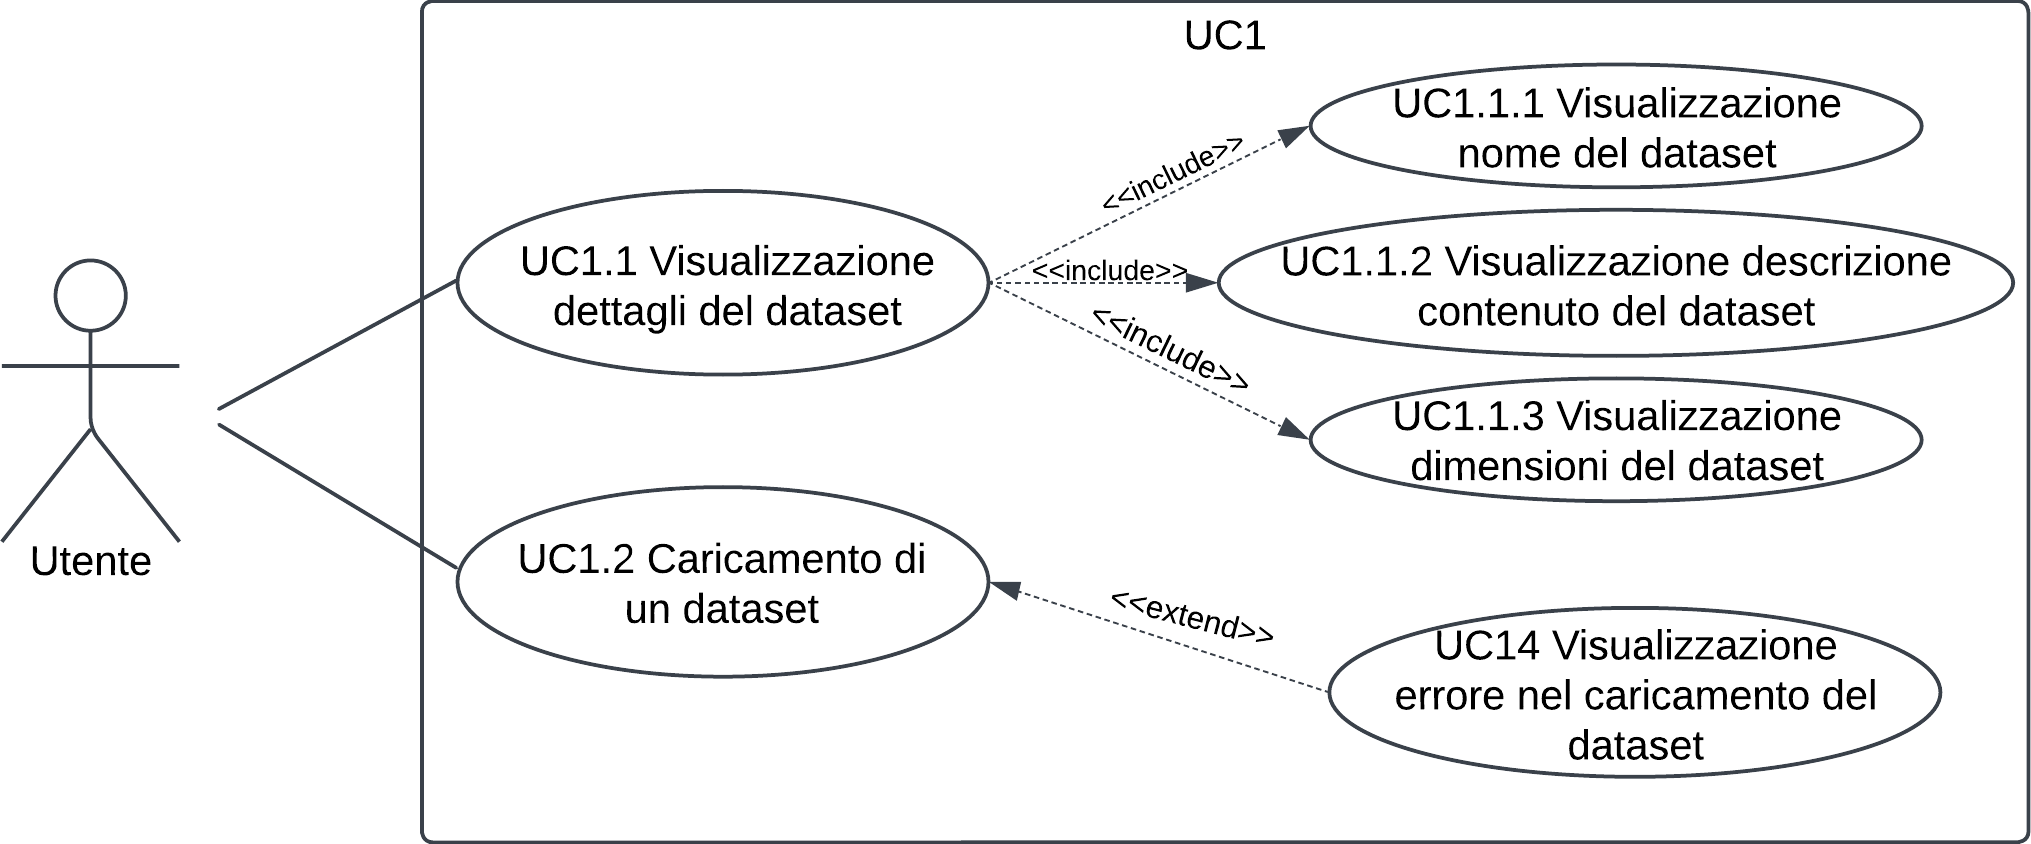
\includegraphics[scale=0.7]{template/images/UC1.png}
        \caption{UC\arabic{UC} - Visualizzazione lista dei dataset disponibili}
    \end{figure}
    \begin{itemize}
        \item \textbf{Attore:} utente;
        \item \textbf{Descrizione:} quando un utente interagisce con l'applicazione web,
        gli viene mostrato un elenco di dataset.\\ Da questa lista, può scegliere il dataset da rappresentare sotto forma di tabella e di grafico 3D.
        \item \textbf{Precondizioni:}
        \begin{itemize}
            \item L'utente ha accesso all'applicazione.
        \end{itemize}
        \item \textbf{Postcondizioni:}
        \begin{itemize}
            \item L'utente vede una lista dei dataset disponibili.
        \end{itemize}
        \item \textbf{Scenario:} 
        \begin{itemize}
            \item L'utente avvia il sistema;
            \item I dataset disponibili vengono presentati tramite un elenco;
            \item L'utente può navigare l'elenco e scegliere il dataset che gli interessa.
        \end{itemize}
    \end{itemize}
    \newpage

    \SubUseCase{Visualizzazione dettagli del dataset}
    \begin{itemize}
        \item \textbf{Attore:} utente;
        \item \textbf{Descrizione:} permette di visualizzare i dettagli del dataset selezionato;
        \item \textbf{Precondizioni:}
        \begin{itemize}
            \item Il sistema ha accesso ai dettagli tecnici e descrittivi del dataset.
        \end{itemize}
        \item \textbf{Postcondizioni:}
        \begin{itemize}
            \item Le informazioni sul dataset vengono mostrate all'utente.
        \end{itemize}
        \item \textbf{Scenario:}
        \begin{itemize}
            \item Il sistema mostra i dettagli dei dataset presenti nell'elenco.
        \end{itemize}
    \end{itemize}

    \SubSubUseCase{Visualizzazione nome del dataset}
    \begin{itemize}
        \item \textbf{Attore:} utente;
        \item \textbf{Descrizione:} l'utente può visualizzare il nome del dataset presente nell'elenco;
        \item \textbf{Precondizioni:}
        \begin{itemize}
            \item Il sistema ha accesso alle informazioni sul dataset.
        \end{itemize}
        \item \textbf{Postcondizioni:}
        \begin{itemize}
            \item Il nome del dataset viene mostrato all'utente.
        \end{itemize}
        \item \textbf{Scenario:}
        \begin{itemize}
            \item Il sistema mostra il nome del dataset.
        \end{itemize}
    \end{itemize}

    \SubSubUseCase{Visualizzazione della descrizione contenuto del dataset}
    \begin{itemize}
        \item \textbf{Attore:} utente;
        \item \textbf{Descrizione:} l'utente può visualizzare una descrizione del contenuto del dataset;
        \item \textbf{Precondizioni:}
        \begin{itemize}
            \item Il sistema ha accesso alle informazioni relative al contenuto del dataset.
        \end{itemize}
        \item \textbf{Postcondizioni:}
        \begin{itemize}
            \item La descrizione del contenuto del dataset viene mostrata all'utente.
        \end{itemize}
        \item \textbf{Scenario:}
        \begin{itemize}
            \item Il sistema mostra una descrizione del contenuto del dataset.
        \end{itemize}
    \end{itemize}

    \SubSubUseCase{Visualizzazione dimensioni tabella}
    \begin{itemize}
        \item \textbf{Attore:} utente;
        \item \textbf{Descrizione:} l'utente può visualizzare le dimensioni della tabella relativa ai dati contenuti nel dataset;
        \item \textbf{Precondizioni:}
        \begin{itemize}
            \item Il sistema ha accesso alle informazioni relative alla dimensione del dataset.
        \end{itemize}
        \item \textbf{Postcondizioni:}
        \begin{itemize}
            \item Le dimensioni della tabella relativa ai dati contenuti nel dataset vengono mostrate all'utente.
        \end{itemize}
        \item \textbf{Scenario:}
        \begin{itemize}
            \item Il sistema mostra le dimensioni della tabella relativa ai dati contenuti nel dataset.
        \end{itemize}
    \end{itemize}

    \SubUseCase{Caricamento di un dataset dall'elenco di quelli disponibili}
    \begin{itemize}
        \item \textbf{Attore:} utente;
        \item \textbf{Descrizione:} consente di caricare il dataset selezionato nell'ambiente 3D dell'applicazione;
        \item \textbf{Precondizioni:}
        \begin{itemize}
            \item L'elenco dei dataset disponibili è stato caricato correttamente;
        \end{itemize}
        \item \textbf{Postcondizioni:}
        \begin{itemize}
            \item Il dataset selezionato viene caricato nel sistema.
        \end{itemize}
        \item \textbf{Scenario:}
        \begin{itemize}
            \item L'utente seleziona un dataset dall'elenco disponibile;
            \item Il sistema prepara i dati per la visualizzazione in forma tabellare e in grafico 3D.
        \end{itemize}
    \end{itemize}
\newpage




\UseCase{Visualizzazione dati in forma tabellare}
\begin{figure}[h!]
    \centering
    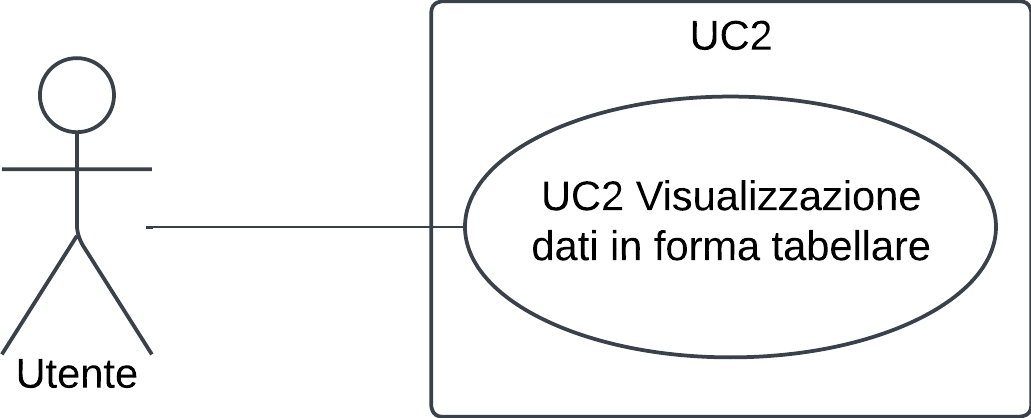
\includegraphics[scale=0.7]{template/images/UC2.png}
    \caption{UC\arabic{UC} - Visualizzazione dati in forma tabellare}
\end{figure}
\begin{itemize}
    \item \textbf{Attore:} utente;
    \item \textbf{Descrizione:} consente di visualizzare il dataset caricato sotto forma di tabella;
    \item \textbf{Precondizioni:}
    \begin{itemize}
        \item Il dataset selezionato è stato caricato correttamente.
    \end{itemize}
    \item \textbf{Postcondizioni:}
    \begin{itemize}
        \item I dati sono mostrati in forma tabellare.
    \end{itemize}
    \item \textbf{Scenario:}
    \begin{itemize}
        \item Il dataset selezionato viene caricato correttamente;
        \item L'applicazione elabora i dati e vengono mostrati in forma tabellare.
    \end{itemize}
\end{itemize}



\UseCase{Visualizzazione dati in forma di grafico a istogramma 3D verticale}
\begin{figure}[h!]
    \centering
    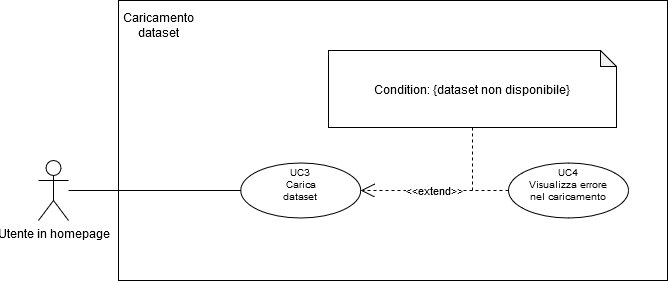
\includegraphics[scale=0.7]{template/images/UC3.png}
    \caption{UC\arabic{UC} - Visualizzazione dati in forma di grafico a istogramma 3D verticale}
\end{figure}
\begin{itemize}
    \item \textbf{Attore:} utente;
    \item \textbf{Descrizione:} consente di visualizzare il dataset caricato sotto forma di grafico a istogramma 3D verticale;
    \item \textbf{Precondizioni:}
    \begin{itemize}
        \item Il dataset selezionato è stato caricato correttamente.
    \end{itemize}
    \item \textbf{Postcondizioni:}
    \begin{itemize}
        \item I dati sono mostrati in forma di grafico a istogramma 3D verticale.
    \end{itemize}
    \item \textbf{Scenario:}
    \begin{itemize}
        \item Il dataset viene caricato correttamente;
        \item L'applicazione elabora i dati e viene creato un grafico a istogramma 3D verticale;
        \item L'interfaccia visualizza il grafico 3D verticale in una vista interattiva, consentendo all'utente di analizzare i dati.
    \end{itemize}
\end{itemize}



\UseCase{Visualizzazione assi}
\begin{itemize}
    \item \textbf{Attore:} utente;
    \item \textbf{Descrizione:} consente di visualizzare dettagliatamente gli assi X, Y e Z del grafico;
    \item \textbf{Precondizioni:} 
    \begin{itemize}
        \item Il grafico 3D è stato generato correttamente;
        \item Gli assi sono correttamente configurati nel sistema.
    \end{itemize}
    \item \textbf{Postcondizioni:}
    \begin{itemize}
        \item Gli assi X, Y e Z sono visibili e ben etichettati.
    \end{itemize}
    \item \textbf{Scenario:}
    \begin{itemize}
        \item L'utente visualizza il grafico 3D;
        \item L'utente visualizza gli assi X,Y e Z.
    \end{itemize}

\end{itemize}
\SubUseCase{Visualizzazione asse X}
\begin{itemize}
    \item \textbf{Attore:} utente;
    \item \textbf{Descrizione:} consente di visualizzare dettagliatamente l'asse X;
    \item \textbf{Precondizioni:} 
    \begin{itemize}
        \item L'asse X è configurato nel grafico.
    \end{itemize}
    \item \textbf{Postcondizioni:} 
    \begin{itemize}
        \item L'asse X è visibile e mostra i valori appropriati.
    \end{itemize}
    \item \textbf{Scenario:} 
    \begin{itemize}
        \item L'utente visualizza il grafico 3D;
        \item L'utente visualizza l'asse X con i valori appropriati.
    \end{itemize}
\end{itemize}
\SubUseCase{Visualizzazione asse Y}
\begin{itemize}
    \item \textbf{Attore:} utente;
    \item \textbf{Descrizione:} consente di visualizzare dettagliatamente l'asse Y;
    \item \textbf{Precondizioni:} 
    \begin{itemize}
        \item L'asse Y è configurato nel grafico.
    \end{itemize}
    \item \textbf{Postcondizioni:} 
    \begin{itemize}
        \item L'asse Y è visibile e mostra i valori appropriati.
    \end{itemize}
    \item \textbf{Scenario:} 
    \begin{itemize}
        \item L'utente visualizza il grafico 3D;
        \item L'utente visualizza l'asse Y con i valori appropriati.
    \end{itemize}
\end{itemize}
\SubUseCase{Visualizzazione asse Z}
\begin{itemize}
    \item \textbf{Attore:} utente;
    \item \textbf{Descrizione:} consente di visualizzare dettagliatamente l'asse Z;
    \item \textbf{Precondizioni:} 
    \begin{itemize}
        \item L'asse Z è configurato nel grafico.
    \end{itemize}
    \item \textbf{Postcondizioni:} 
    \begin{itemize}
        \item L'asse Z è visibile e mostra i valori appropriati.
    \end{itemize}
    \item \textbf{Scenario:} 
    \begin{itemize}
        \item L'utente visualizza il grafico 3D;
        \item L'utente visualizza l'asse Z con i valori appropriati.
    \end{itemize}
\end{itemize}



\UseCase{Visualizzazione legenda}
\begin{itemize}
    \item \textbf{Attore:} utente;
    \item \textbf{Descrizione:} consente di visualizzare una legenda con dettagli e informazioni sul grafico;
    \item \textbf{Precondizioni:} 
    \begin{itemize}
        \item Il grafico 3D è stato generato correttamente;
        \item Il sistema dispone delle informazioni necessarie per creare una legenda.
    \end{itemize}
    \item \textbf{Postcondizioni:}
    \begin{itemize}
        \item La legenda è visibile e fornisce informazioni dettagliate che aiutano l'utente a comprendere i dati rappresentati.
    \end{itemize}
    \item \textbf{Scenario:} 
    \begin{itemize}
        \item Il grafico viene generato correttamente;
        \item La legenda relativa al grafico è visibile.
    \end{itemize}
\end{itemize}



\UseCase{Pan}
\begin{figure}[h!]
    \centering
    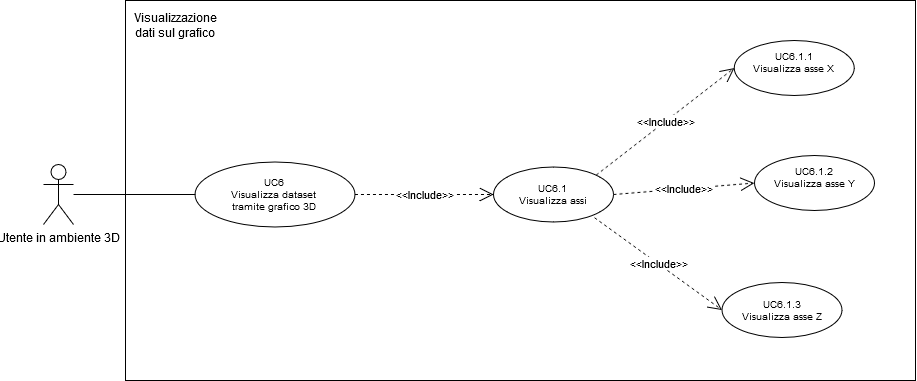
\includegraphics[scale=0.7]{template/images/UC6.png}
    \caption{UC\arabic{UC} - PAN}
\end{figure}
\begin{itemize}
    \item \textbf{Attore:} utente;
    \item \textbf{Descrizione:} l'utente sposta la visualizzazione del grafico 3D lungo il piano XY senza modificare l'orientamento della camera;
    \item \textbf{Precondizioni:}
    \begin{itemize}
        \item L'utente sta visualizzando il grafico 3D;
        \item Il sistema ha abilitato la funzionalità di interazione pan.
    \end{itemize}
    \item \textbf{Postcondizioni}:
    \begin{itemize}
        \item La vista della scena 3D è stata spostata nella direzione indicata dall'utente.
    \end{itemize}
    \item \textbf{Scenario:}
    \begin{itemize}
        \item L'utente visualizza il grafico 3D nell'interfaccia;
        \item L'utente interagisce con il grafico utilizzando il mouse (trascinamento);
        \item Il sistema interpreta il comando di spostamento e aggiorna la posizione del grafico lungo il piano XY;
        \item La nuova vista viene aggiornata in tempo reale e mostrata all'utente.
    \end{itemize}
\end{itemize}



\UseCase{Rotazione camera}
\begin{figure}[h!]
    \centering
    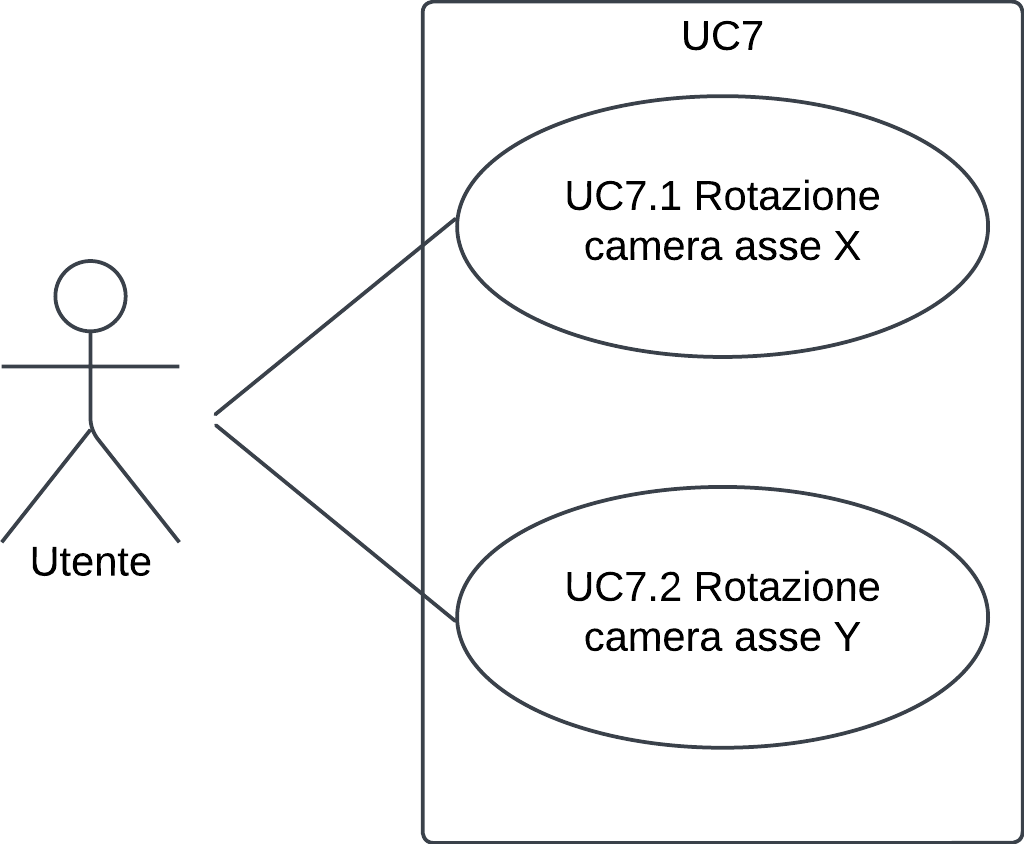
\includegraphics[scale=0.7]{template/images/UC7_7.1_7.2.png}
    \caption{UC\arabic{UC} - Rotazione camera}
\end{figure}
\begin{itemize}
    \item \textbf{Attore:} utente;
    \item \textbf{Descrizione:} l'utente ruota la visualizzazione del grafico 3D modificando l'orientamento della camera lungo uno o più assi. La rotazione consente di analizzare il grafico da diverse angolazioni;
    \item \textbf{Precondizioni:} 
    \begin{itemize}
        \item L'utente sta visualizzando il grafico 3D nell'interfaccia;
        \item Il sistema ha abilitato le funzionalità di interazione con la camera.
    \end{itemize}
    \item \textbf{Postcondizioni:} 
    \begin{itemize}
        \item La visualizzazione del grafico è stata aggiornata in base alla rotazione effettuata dall'utente.
    \end{itemize}
    \item \textbf{Scenario:} 
    \begin{itemize}
        \item L'utente interagisce con il grafico 3D usando i comandi per ruotare la visualizzazione. Il sistema aggiorna in tempo reale l'orientamento della camera, mostrando il grafico da una nuova angolazione.
    \end{itemize}
    
\end{itemize}
\SubUseCase{Rotazione camera asse X}
\begin{itemize}
    \item \textbf{Attore:} utente;
    \item \textbf{Descrizione:} l'utente ruota la visualizzazione del grafico 3D attorno all'asse X, modificando l'altezza della prospettiva.
    \item \textbf{Precondizioni:} 
    \begin{itemize}
        \item L'utente sta visualizzando il grafico 3D nell'interfaccia;
        \item Il sistema ha abilitato le funzionalità di interazione con la camera.
    \end{itemize}
    \item \textbf{Postcondizioni:} 
    \begin{itemize}
        \item La camera è stata ruotata attorno all'asse X, aggiornando la vista in tempo reale.
    \end{itemize}
    \item \textbf{Scenario:}
    \begin{itemize}
        \item L'utente usa comandi per spostare la vista verso l'alto o verso il basso. Il sistema ruota la camera attorno all'asse X, consentendo di osservare il grafico da un'angolazione più alta o più bassa.
    \end{itemize}
    
\end{itemize}
\SubUseCase{Rotazione camera asse Y}
\begin{itemize}
    \item \textbf{Attore:} utente;
    \item \textbf{Descrizione:} l'utente ruota la visualizzazione del grafico 3D attorno all'asse Y, modificando l'orientamento laterale della prospettiva;
    \item \textbf{Precondizioni:} 
    \begin{itemize}
        \item L'utente sta visualizzando il grafico 3D nell'interfaccia;
        \item Il sistema ha abilitato le funzionalità di interazione con la camera.
    \end{itemize}
    \item \textbf{Postcondizioni:} 
    \begin{itemize}
        \item La camera è stata ruotata attorno all'asse Y, aggiornando la vista in tempo reale.
    \end{itemize}
    \item \textbf{Scenario:} 
    \begin{itemize}
        \item L'utente usa comandi per spostare la vista verso destra o sinistra. Il sistema ruota la camera attorno all'asse Y, consentendo di osservare il grafico da angolazioni diverse lateralmente.
    \end{itemize}
\end{itemize}



\UseCase{Movimenti direzionali}
\begin{figure}[h!]\centering
    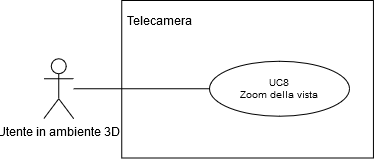
\includegraphics[scale=0.7]{template/images/UC8.png}
    \caption{UC\arabic{UC} - Movimenti direzionali}
\end{figure}
\begin{itemize}    
    \item \textbf{Attore:} utente;
    \item \textbf{Descrizione:} Compiere movimenti direzionali significa che, in ambiente di visualizzazione del grafico 3D, l'utente può interagire con il grafico compiendo degli spostamenti lungo i tre assi principali tramite comandi opportuni.
    \item \textbf{Precondizioni:}    
        \begin{itemize}
            \item Il caricamento del dataset è avvenuto con successo;
            \item La generazione dell'ambiente 3D e del relativo grafico non hanno riscontrato errori;
            \item Vengono eseguiti i comandi opportuni per i vari spostamenti.
        \end{itemize}    
    \item \textbf{Postcondizioni:}
        \begin{itemize}
            \item La telecamera che inquadra il grafico nell'ambiente 3D si troverà in una posizione diversa da quella in cui si trovava prima di compiere lo spostamento.
        \end{itemize}    
    \item \textbf{Scenario:} 
        \begin{itemize}
            \item L'utente interagisce con l'ambiente 3D per compiere un movimento direzionale.
        \end{itemize}
\end{itemize}
\SubUseCase{Movimento direzionale asse X}
\begin{itemize}    
    \item \textbf{Attore:} utente;
    \item \textbf{Descrizione:} L'utente interagisce opportunamente con l'ambiente 3D per spostarsi lungo l'asse X.
    \item \textbf{Precondizioni:}    
        \begin{itemize}
            \item Il caricamento del dataset è avvenuto con successo;
            \item La generazione dell'ambiente 3D e del relativo grafico non hanno riscontrato errori;
            \item Vengono eseguiti i comandi opportuni per lo spostamento lungo l'asse X.
        \end{itemize}    
    \item \textbf{Postcondizioni:}
        \begin{itemize}
            \item La telecamera che inquadra il grafico nell'ambiente 3D si troverà in una posizione diversa da quella in cui si trovava prima di compiere lo spostamento rispetto all'asse X.
        \end{itemize}    
    \item \textbf{Scenario:} 
        \begin{itemize}
            \item L'utente interagisce con l'ambiente 3D per compiere un movimento direzionale lungo l'asse X.
        \end{itemize}
\end{itemize}
\SubUseCase{Movimento direzionale asse Y}
\begin{itemize}    
    \item \textbf{Attore:} utente;
    \item \textbf{Descrizione:} L'utente interagisce opportunamente con l'ambiente 3D per spostarsi lungo l'asse Y.
    \item \textbf{Precondizioni:}   
        \begin{itemize}
            \item Il caricamento del dataset è avvenuto con successo;
            \item La generazione dell'ambiente 3D e del relativo grafico non hanno riscontrato errori;
            \item Vengono eseguiti i comandi opportuni per lo spostamento lungo l'asse Y.
        \end{itemize}    
    \item \textbf{Postcondizioni:}
        \begin{itemize}
            \item La telecamera che inquadra il grafico nell'ambiente 3D si troverà in una posizione diversa da quella in cui si trovava prima di compiere lo spostamento rispetto all'asse Y.
        \end{itemize}    
    \item \textbf{Scenario:} 
        \begin{itemize}
            \item L'utente interagisce con l'ambiente 3D per compiere un movimento direzionale lungo l'asse Y.
        \end{itemize}
\end{itemize}
\SubUseCase{Movimento direzionale asse Z}
\begin{itemize}    
    \item \textbf{Attore:} utente;
    \item \textbf{Descrizione:} L'utente interagisce opportunamente con l'ambiente 3D per spostarsi lungo l'asse Z.
    \item \textbf{Precondizioni:}    
        \begin{itemize}
            \item Il caricamento del dataset è avvenuto con successo;
            \item La generazione dell'ambiente 3D e del relativo grafico non hanno riscontrato errori;
            \item Vengono eseguiti i comandi opportuni per lo spostamento lungo l'asse Z.
        \end{itemize}    
    \item \textbf{Postcondizioni:}
        \begin{itemize}
            \item La telecamera che inquadra il grafico nell'ambiente 3D si troverà in una posizione diversa da quella in cui si trovava prima di compiere lo spostamento rispetto all'asse Z.
        \end{itemize}    
    \item \textbf{Scenario:} 
        \begin{itemize}
            \item L'utente interagisce con l'ambiente 3D per compiere un movimento direzionale lungo l'asse Z.
        \end{itemize}
\end{itemize}



\UseCase{Riposizionamento iniziale}
\begin{figure}[h!]\centering
    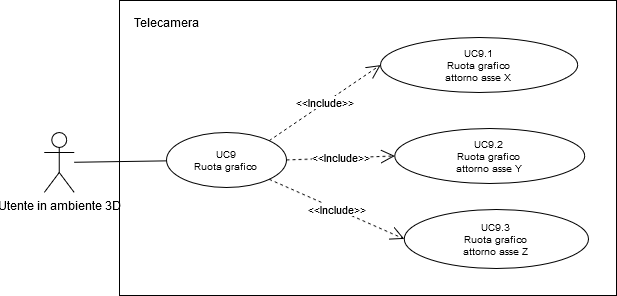
\includegraphics[scale=0.7]{template/images/UC9.png}
    \caption{UC\arabic{UC} - Riposizionamento iniziale}
\end{figure}
\begin{itemize}    
    \item \textbf{Attore:} utente;
    \item \textbf{Descrizione:} Riposizionare inizialmente la telecamera significa ripristinare la sua posizione e angolazione alla configurazione di partenza, annullando qualsiasi modifica apportata successivamente all'inizializzazione dell'ambiente 3D.
    \item \textbf{Precondizioni:}    
        \begin{itemize}
            \item Il caricamento del dataset è avvenuto con successo;
            \item La generazione dell'ambiente 3D e del relativo grafico non hanno riscontrato errori;
            \item Viene eseguito il comando opportuno per il riposizionamento iniziale.
        \end{itemize}    
    \item \textbf{Postcondizioni:}
        \begin{itemize}
            \item La posizione e angolazione della telecamera corrispondono alla configurazione di iniziale, uguale a quella di inizializzazione dell'ambiente 3D.
        \end{itemize}    
    \item \textbf{Scenario:} 
        \begin{itemize}
            \item L'utente interagisce con l'interfaccia per ripristinare la posizione e angolazione della telecamera ai valori iniziali.
        \end{itemize}
\end{itemize}



\UseCase{Visualizzazione dei valori di una barra del grafico}
\begin{figure}[h!]\centering
    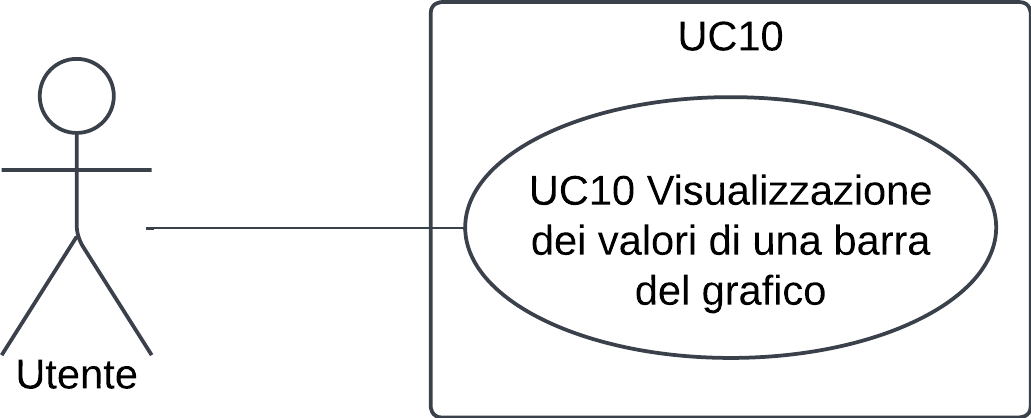
\includegraphics[scale=0.7]{template/images/UC10.png}
    \caption{UC\arabic{UC} - Visualizzazione dei valori di una barra del grafico}
\end{figure}
\begin{itemize}    
    \item \textbf{Attore:} utente;
    \item \textbf{Descrizione:} L'utente, tramite interazione opportuna, può selezionare una barra del grafico all'interno dell'ambiente 3D per visualizzarne i rispettivi valori.
    \item \textbf{Precondizioni:}    
        \begin{itemize}
            \item Il caricamento del dataset è avvenuto con successo;
            \item La generazione dell'ambiente 3D e del relativo grafico non hanno riscontrato errori;
            \item Viene eseguita l'interazione opportuna da parte dell'utente per la selezione della barra del grafico.
        \end{itemize}    
    \item \textbf{Postcondizioni:}
        \begin{itemize}
            \item Vengono visualizzati a schermo i valori della barra del grafico selezionata.
        \end{itemize}    
    \item \textbf{Scenario:} 
        \begin{itemize}
            \item L'utente interagisce con l'ambiente 3D e seleziona una barra del grafico per far apparire a schermo i valori.
        \end{itemize}
\end{itemize}



\UseCase{Selezione elementi}
\begin{figure}[h!]\centering
    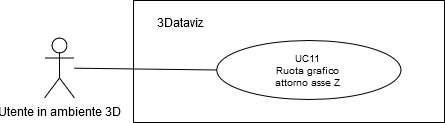
\includegraphics[scale=0.7]{template/images/UC11.png}
    \caption{UC\arabic{UC} - Selezione elementi}
\end{figure}
\begin{itemize}    
    \item \textbf{Attore:} utente;
    \item \textbf{Descrizione:} L'utente, tramite interazione opportuna, può selezionare una barra del grafico all'interno dell'ambiente 3D oppure una singola cella nella tabella.
    \item \textbf{Precondizioni:}    
        \begin{itemize}
            \item Il caricamento del dataset è avvenuto con successo;
            \item La generazione dell'ambiente 3D e del relativo grafico non hanno riscontrato errori;
            \item La generazione della tabella non ha riscontrato errori;
            \item Viene eseguita l'interazione opportuna da parte dell'utente per la selezione.
        \end{itemize}    
    \item \textbf{Postcondizioni:}
        \begin{itemize}
            \item Viene evidenziata la selezione.
        \end{itemize}    
    \item \textbf{Scenario:} 
        \begin{itemize}
            \item L'utente interagisce con l'ambiente 3D e seleziona una barra del grafico oppure seleziona una cella della tabella.
        \end{itemize}
\end{itemize}

\pagebreak

\SubUseCase{Selezione di un elemento del grafico}
\begin{figure}[h!]\centering
    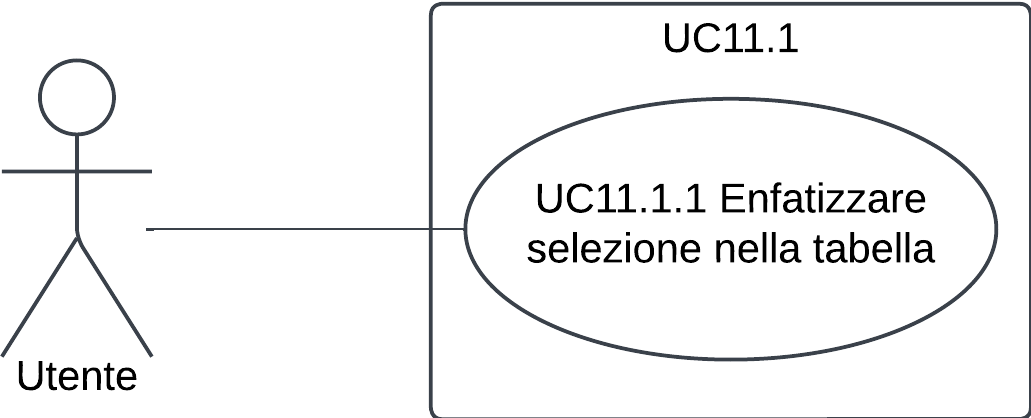
\includegraphics[scale=0.7]{template/images/UC11.1.png}
    \caption{UC\arabic{UC}.\arabic{SUC} - Selezione di un elemento del grafico}
\end{figure}
\begin{itemize}    
    \item \textbf{Attore:} utente;
    \item \textbf{Descrizione:} L'utente può selezionare una barra del grafico 3D.
    \item \textbf{Precondizioni:}    
        \begin{itemize}
            \item Il caricamento del dataset è avvenuto con successo;
            \item La generazione dell'ambiente 3D e del relativo grafico non hanno riscontrato errori;
            \item Viene eseguita l'interazione opportuna da parte dell'utente per la selezione.
        \end{itemize}    
    \item \textbf{Postcondizioni:}
        \begin{itemize}
            \item Viene evidenziata della barra del grafico 3D.
        \end{itemize}    
    \item \textbf{Scenario:} 
        \begin{itemize}
            \item L'utente interagisce con il grafico 3D e seleziona una barra.
        \end{itemize}
\end{itemize}
\SubSubUseCase{Enfatizzazione della selezione nella tabella}
\begin{itemize}    
    \item \textbf{Attore:} utente;
    \item \textbf{Descrizione:} Viene evidenziata in maniera opportuna nella tabella la selezione compiuta dall'utente nel grafico 3D.
    \item \textbf{Precondizioni:}    
        \begin{itemize}
            \item Il caricamento del dataset è avvenuto con successo;
            \item La generazione della tabella non ha riscontrato errori;
            \item Viene eseguita l'interazione opportuna da parte dell'utente per la selezione.
        \end{itemize}    
    \item \textbf{Postcondizioni:}
        \begin{itemize}
            \item Viene evidenziata la cella nella tabella.
        \end{itemize}    
    \item \textbf{Scenario:} 
        \begin{itemize}
            \item L'utente interagisce con il grafico 3D, evidenziando la corrispondente cella della tabella.
        \end{itemize}
\end{itemize}

\pagebreak

\SubUseCase{Selezione di una cella della tabella}
\begin{figure}[h!]\centering
    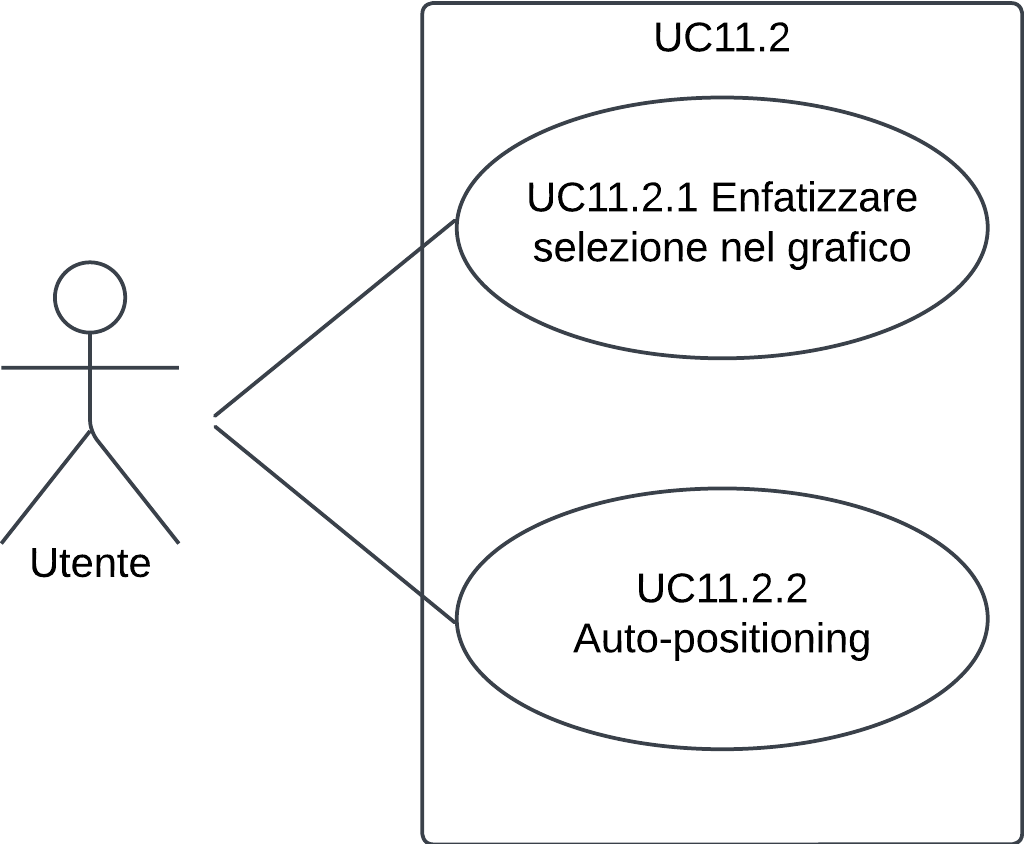
\includegraphics[scale=0.7]{template/images/UC11.2.png}
    \caption{UC\arabic{UC}.\arabic{SUC}: Selezione di una cella della tabella}
\end{figure}
\begin{itemize}    
    \item \textbf{Attore:} utente;
    \item \textbf{Descrizione:} L'utente può selezionare una cella all'interno della tabella.
    \item \textbf{Precondizioni:}    
        \begin{itemize}
            \item Il caricamento del dataset è avvenuto con successo;
            \item La generazione della tabella non ha riscontrato errori;
            \item Viene eseguita l'interazione opportuna da parte dell'utente per la selezione della cella.
        \end{itemize}    
    \item \textbf{Postcondizioni:}
        \begin{itemize}
            \item Viene evidenziata la cella della tabella.
        \end{itemize}    
    \item \textbf{Scenario:} 
        \begin{itemize}
            \item L'utente interagisce con la tabella selezionando una cella la quale verrà evidenziata.
        \end{itemize}
\end{itemize}
\SubSubUseCase{Enfatizzazione selezione nel grafico}
\begin{itemize}    
    \item \textbf{Attore:} utente;
    \item \textbf{Descrizione:} Viene evidenziata in maniera opportuna nel grafico 3D la selezione compiuta dall'utente nella tabella.
    \item \textbf{Precondizioni:}    
        \begin{itemize}
            \item Il caricamento del dataset è avvenuto con successo;
            \item La generazione dell'ambiente 3D e del relativo grafico non hanno riscontrato errori;
            \item Viene eseguita l'interazione opportuna da parte dell'utente per la selezione.
        \end{itemize}    
    \item \textbf{Postcondizioni:}
        \begin{itemize}
            \item Viene evidenziata la barra del grafico 3D.
        \end{itemize}    
    \item \textbf{Scenario:} 
        \begin{itemize}
            \item L'utente interagisce con una cella della tabella, evidenziando la corrispondente barra del grafico 3D.
        \end{itemize}
\end{itemize}
\SubSubUseCase{Auto-positioning}
\begin{itemize}    
    \item \textbf{Attore:} utente;
    \item \textbf{Descrizione:} In seguito alla selezione di una cella, la vista si sposta sulla corrispondente barra del grafico 3D, centrandola sullo schermo.
    \item \textbf{Precondizioni:}    
        \begin{itemize}
            \item Il caricamento del dataset è avvenuto con successo;
            \item La generazione dell'ambiente 3D e del relativo grafico non hanno riscontrato errori;
            \item Viene richiesta un'operazione di auto-positioning.
        \end{itemize}    
    \item \textbf{Postcondizioni:}
        \begin{itemize}
            \item La telecamera e la relativa inquadratura saranno in una posizione diversa da quella iniziale e avranno inoltre in primo piano la barra selezionata del grafico 3D.
        \end{itemize}    
    \item \textbf{Scenario:} 
        \begin{itemize}
            \item L'utente seleziona una cella della tabella e la telecamera nell'ambiente 3D si sposta di conseguenza inquadrando la corrispettiva barra del grafico.
        \end{itemize}
\end{itemize}




\UseCase{Modifica trasparenza barra del grafico}
\begin{figure}[h!]\centering
    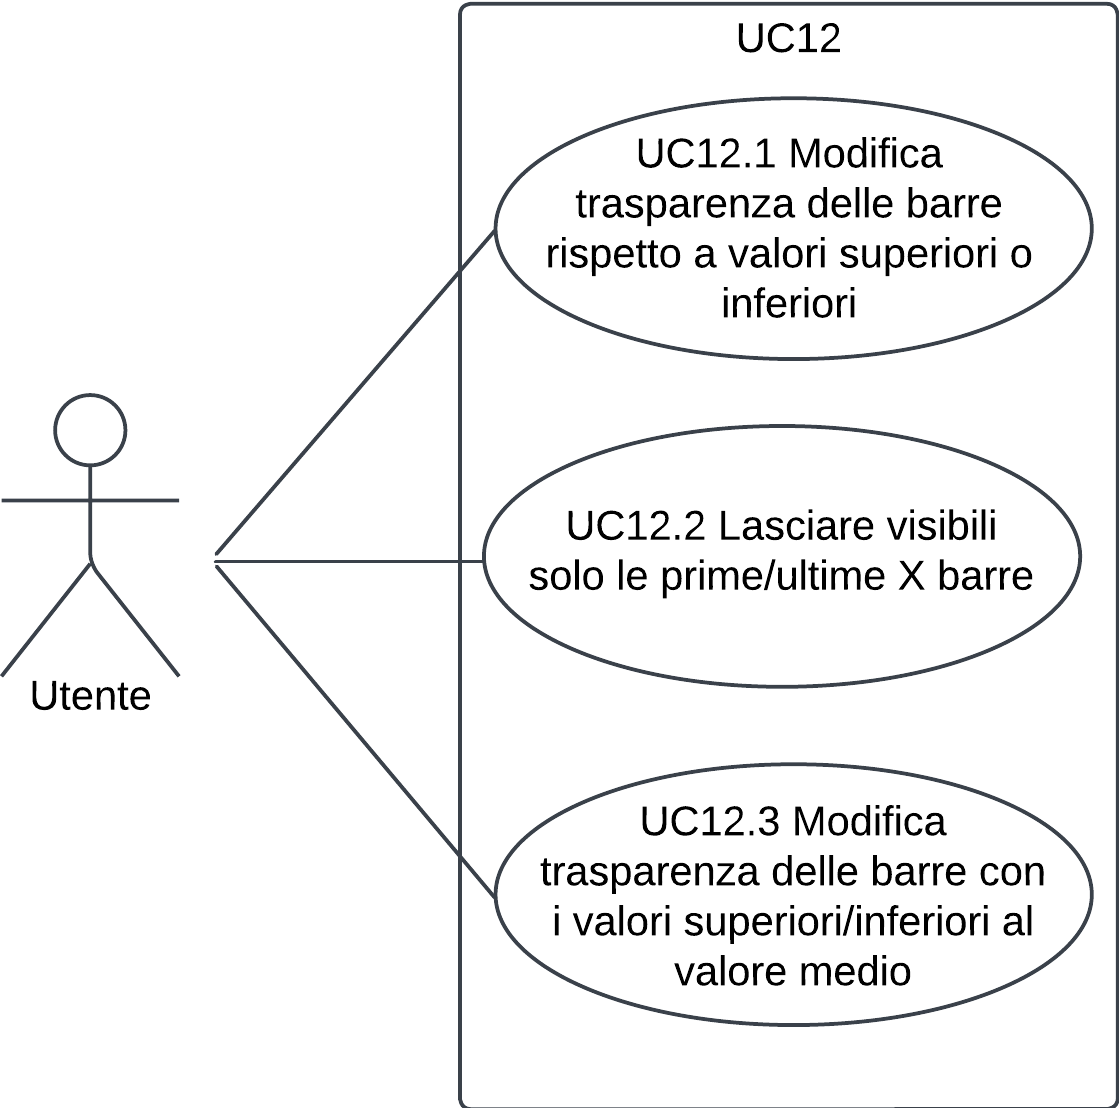
\includegraphics[scale=0.7]{template/images/UC12.png}
    \caption{UC\arabic{UC} - Modifica trasparenza barra del grafico}
\end{figure}
\begin{itemize}    
    \item \textbf{Attore:} utente;
    \item \textbf{Descrizione:} Viene aumentata la trasparenza di una barra del grafico all'interno dell'ambiente 3D.
    \item \textbf{Precondizioni:}    
        \begin{itemize}
            \item Il caricamento del dataset è avvenuto con successo;
            \item La generazione dell'ambiente 3D e del relativo grafico non hanno riscontrato errori.
        \end{itemize}    
    \item \textbf{Postcondizioni:}
        \begin{itemize}
            \item Il valore di trasparenza delle altre barre del grafico 3D è maggiore rispetto a quello delle altre.
        \end{itemize}    
    \item \textbf{Scenario:} 
        \begin{itemize}
            \item L'utente evidenzia una determinata barra del grafico viene aumentato il valore di trasparenza a tutte le altre.
        \end{itemize}
\end{itemize}
\SubUseCase{Modifica trasparenza delle barre rispetto a valori superiori o inferiori}
\begin{itemize}    
    \item \textbf{Attore:} utente;
    \item \textbf{Descrizione:} L'utente può stabilire un valore limite al di sopra o al di sotto del quale alcune barre verranno evidenziate.
    \item \textbf{Precondizioni:}    
        \begin{itemize}
            \item Il caricamento del dataset è avvenuto con successo;
            \item La generazione dell'ambiente 3D e del relativo grafico non hanno riscontrato errori;
            \item La generazione dell'interfaccia non ha riscontrato errori;
            \item L'utente imposta correttamente tutti i parametri necessari.
        \end{itemize}    
    \item \textbf{Postcondizioni:}
        \begin{itemize}
            \item Ogni barra selezionata nel grafico 3D viene resa più visibile rendendo le altre barre più trasparenti.
        \end{itemize}    
    \item \textbf{Scenario:} 
        \begin{itemize}
            \item L'utente interagisce con l'interfaccia selezionando il numero di barre con i valori più elevati o più bassi da evidenziare nel grafico 3D.
        \end{itemize}
\end{itemize}
\SubUseCase{Lasciare visibili solo le prime/ultime X barre}
\begin{itemize}    
    \item \textbf{Attore:} utente;
    \item \textbf{Descrizione:} L'utente può selezionare quante barre con i valori più elevati o più bassi evidenziare.
    \item \textbf{Precondizioni:}    
        \begin{itemize}
            \item Il caricamento del dataset è avvenuto con successo;
            \item La generazione dell'ambiente 3D e del relativo grafico non hanno riscontrato errori;
            \item La generazione dell'interfaccia non ha riscontrato errori;
            \item L'utente imposta correttamente tutti i parametri necessari.
        \end{itemize}    
    \item \textbf{Postcondizioni:}
        \begin{itemize}
            \item Ogni barra selezionata nel grafico 3D viene resa più visibile rendendo le altre barre più trasparenti.
        \end{itemize}    
    \item \textbf{Scenario:} 
        \begin{itemize}
            \item L'utente interagisce con l'interfaccia selezionando il numero di barre con i valori più elevati o più bassi da evidenziare nel grafico 3D.
        \end{itemize}
\end{itemize}
\SubUseCase{Modifica trasparenza delle barre con i valori superiori/inferiori al valore medio}
\begin{itemize}    
    \item \textbf{Attore:} utente;
    \item \textbf{Descrizione:} L'utente può scegliere se evidenziare nel grafico 3D le barre il quale valore è superiore o inferiore al valore medio.
    \item \textbf{Precondizioni:}    
        \begin{itemize}
            \item Il caricamento del dataset è avvenuto con successo;
            \item La generazione dell'ambiente 3D e del relativo grafico non hanno riscontrato errori;
            \item La generazione dell'interfaccia non ha riscontrato errori;
            \item L'utente imposta correttamente tutti i parametri necessari.
        \end{itemize}    
    \item \textbf{Postcondizioni:}
        \begin{itemize}
            \item Ogni barra con il rispettivo valore superiore/inferiore al valore medio verrà opacizzata.
        \end{itemize}    
    \item \textbf{Scenario:} 
        \begin{itemize}
            \item L'utente interagisce con l'interfaccia per evidenziare nel grafico 3D solo le barre con un valore superiore o inferiore al valore medio.
        \end{itemize}
\end{itemize}




\UseCase{Visualizzazione di un piano parallelo alla base}
\begin{figure}[h!]\centering
    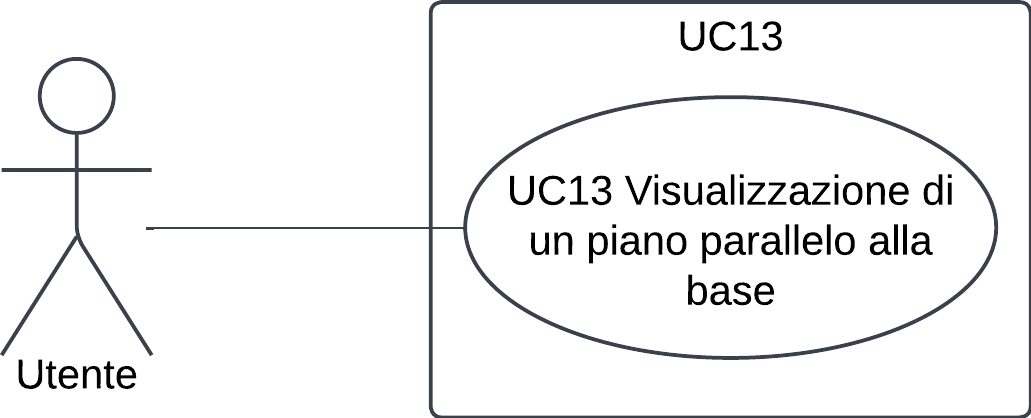
\includegraphics[scale=0.7]{template/images/UC13.png}
    \caption{UC\arabic{UC} - Visualizzazione di un piano parallelo alla base}
\end{figure}
\begin{itemize}    
    \item \textbf{Attore:} utente;
    \item \textbf{Descrizione:} Un piano, parallelo alla base, viene inserito nel grafico 3D per evidenziare un valore di interesse, scelto dall'utente tra quelli ricavabili dai dati. Questo piano offre una rappresentazione visiva immediata del valore selezionato.
    \item \textbf{Precondizioni:}    
        \begin{itemize}
            \item Il caricamento del dataset è avvenuto con successo;
            \item La generazione dell'ambiente 3D e del relativo grafico non hanno riscontrato errori.
        \end{itemize}    
    \item \textbf{Postcondizioni:}
        \begin{itemize}
            \item Viene generato un piano, nel grafico 3D, parallelo alla base che evidenzia il valore di interesse scelto dall'utente.
        \end{itemize}    
    \item \textbf{Scenario:} 
        \begin{itemize}
            \item L'utente può evidenziare un determinato valore di interesse (ad esempio il valore medio) ed esso sarà rappresentato nel grafico dal piano generato.
        \end{itemize}
\end{itemize}

\pagebreak


\UseCase{Visualizzazione errore nel caricamento del dataset}
\begin{figure}[h!]\centering
    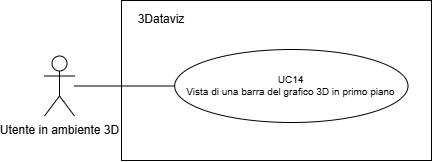
\includegraphics[scale=0.7]{template/images/UC14.png}
    \caption{UC\arabic{UC}: Visualizzazione errore nel caricamento del dataset}
\end{figure}
\begin{itemize}    
    \item \textbf{Attore:} utente;
    \item \textbf{Descrizione:} L'utente visualizza un messaggio di errore dovuto al caricamento del dataset.
    \item \textbf{Precondizioni:}    
        \begin{itemize}
            \item L'utente ha selezionato il dataset da caricare;
            \item Il caricamento del dataset non è andato a buon fine.
        \end{itemize}    
    \item \textbf{Postcondizioni:}
        \begin{itemize}
            \item Viene visualizzato a schermo un messaggio di errore in seguito ad uno o più problemi riscontrati durante il caricamento del dataset selezionato.
        \end{itemize}    
    \item \textbf{Scenario:} 
        \begin{itemize}
            \item L'utente, in seguito al fallimento del caricamento del dataset selezionato, visualizza il messaggio di errore.
        \end{itemize}
\end{itemize}

\pagebreak

\newcommand{\requirementsTable}[1]{

\renewcommand{\arraystretch}{1.5}
\rowcolors{2}{pari}{dispari}
\begin{longtable}{ %0.87
		>{\centering}M{0.15\textwidth} 
		>{\centering}M{0.5\textwidth}
		>{\centering}M{0.20\textwidth}
		>{\centering\arraybackslash}M{0.15\textwidth} 
		 }
	\rowcolorhead
	\headertitle{Requisito} &
	\centering \headertitle{Descrizione} &	
	\headertitle{Fonte}
	\endfirsthead	
	\endhead
	
	#1

\end{longtable}
\vspace{2em}

}

\newcommand{\SrcToReqTable}[1]{

\renewcommand{\arraystretch}{1.5}
\rowcolors{2}{pari}{dispari}
\begin{longtable}{ %0.87
		>{\centering}M{0.5\textwidth} 
		>{\centering\arraybackslash}M{0.20\textwidth} 
		 }
	\rowcolorhead
	\headertitle{Fonte} &
	\centering\headertitle{Requisito}
	\endfirsthead	
	\endhead
	
	#1

\end{longtable}
\vspace{2em}

}

\newcommand{\ReqToUCTable}[1]{

\renewcommand{\arraystretch}{1.5}
\rowcolors{2}{pari}{dispari}
\begin{longtable}{ %0.87
		>{\centering}M{0.5\textwidth} 
		>{\centering\arraybackslash}M{0.20\textwidth} 
		 }
	\rowcolorhead
	\headertitle{Requisito} &
	\centering\headertitle{Fonte}
	\endfirsthead	
	\endhead
	
	#1

\end{longtable}
\vspace{2em}

}

\newcommand{\requirementsSummaryTable}[1]{

\renewcommand{\arraystretch}{1.5}
\rowcolors{2}{pari}{dispari}
\begin{longtable}{ %0.87
		>{\centering}M{0.3\textwidth} 
		>{\centering}M{0.15\textwidth}
		>{\centering}M{0.15\textwidth}
		>{\centering}M{0.15\textwidth}
		>{\centering\arraybackslash}M{0.15\textwidth} 
		 }
	\rowcolorhead
	\headertitle{Tipologia} &
	\centering \headertitle{Obbligatorio} &	
	\headertitle{Desiderabile} &
	\headertitle{Opzionale} &
	\headertitle{Totale}
	\endfirsthead	
	\endhead
	
	#1

\end{longtable}
\vspace{2em}

}

\section{Requisiti}
\subsection{Introduzione}
Sono stati definiti dei requisiti codificati in base all’ambito di competenza e ad un numero seriale per
tenerne meglio traccia, inoltre nelle tabelle sottostanti sono fornite di descrizione e classificazione di ciascun
requisito. Il codice di ciascuno requisito è formato da:
\begin{itemize}
    \item \textbf{R} : Sta per requisito e serve a definire il dominio del codice rendendo subito intuibile che si tratti di
    un requisito;
    \item Lettera di tipologia:
    \begin{itemize}
        \item \textbf{F}: Funzionale;
        \item \textbf{Q}: Di qualità;
        \item \textbf{D}: Di vincolo;
        \item \textbf{P}: Prestazionale;
    \end{itemize}
\end{itemize}
\subsection{Requisiti funzionali}
\requirementsTable{
    RF1 & L’utente deve poter visualizzare i dataset proposti & Obbligatorio & UC1 \tabularnewline
    RF1.1 & L’utente deve poter visualizzare i dettagli dataset selezionato & Obbligatorio & UC1.1\par UC1.1.1\par UC1.1.2\par UC1.1.3\par \tabularnewline
    RF1.2 & L’utente deve poter caricare il dataset selezionato & Obbligatorio & UC1.2 \tabularnewline

    RF2 & L’utente deve poter visualizzare i dati del dataset selezionato in forma tabellare & Obbligatorio & UC2 \tabularnewline
    
    RF3 & L’utente deve poter visualizzare i dati del dataset selezionato in forma di grafico tridimensionale a barre verticali & Obbligatorio & UC3 \tabularnewline
    
    RF4 & L’utente deve poter visualizzare gli assi del grafico tridimensionale  & Obbligatorio & UC4 \tabularnewline
    RF4.1 & L’utente deve poter visualizzare l`asse globale X del grafico tridimensionale  & Obbligatorio & UC4.1 \tabularnewline
    RF4.2 & L’utente deve poter visualizzare l`asse globale Y del grafico tridimensionale  & Obbligatorio & UC4.2 \tabularnewline
    RF4.3 & L’utente deve poter visualizzare l`asse globale Z del grafico tridimensionale  & Obbligatorio & UC4.3 \tabularnewline
    
    RF5 & L’utente deve poter visualizzare la legenda del grafico tridimensionale  & Obbligatorio & UC5 \tabularnewline
 
    RF6 & L’utente deve poter effettuare un`azione di pan nell` ambiente, spostando la telecamera sugli assi locali Y e X & Obbligatorio & UC6 \tabularnewline
    
    RF7 & L’utente deve poter ruotare la telecamera a suo piacimento per visualizzare meglio il grafico tridimensionale & Obbligatorio & UC7 \tabularnewline
    RF7.1 & L’utente deve poter ruotare la telecamera attorno all`asse globale X & Obbligatorio & UC7.1 \tabularnewline
    RF7.2 & L’utente deve poter ruotare la telecamera attorno all`asse globale Y & Obbligatorio & UC7.2 \tabularnewline
    
    RF8 & L’utente deve poter muovere la telecamera all`interno dell` ambiente & Obbligatorio & UC8 \tabularnewline
    RF8.1 & L’utente deve poter muovere la telecamera sull`asse globale X & Obbligatorio & UC8.1 \tabularnewline
    RF8.2 & L’utente deve poter muovere la telecamera sull`asse globale Y & Obbligatorio & UC8.2 \tabularnewline
    RF8.3 & L’utente deve poter muovere la telecamera sull`asse globale Z & Obbligatorio & UC8.3 \tabularnewline
    
    RF9 & L’utente deve poter riposizionare la telecamera alla sua posizione iniziale & Obbligatorio & UC9 \tabularnewline
    
    RF10 & L’utente deve poter visualizzare i valori del dataset selezionando le barre opportune verticali del grafico tridimensionale & Obbligatorio & UC10 \tabularnewline
    
    RF11 & L’utente deve poter selezionare elementi rappresentanti i dati del dataset & Obbligatorio & UC11 \tabularnewline
    RF11.1 & L’utente deve poter selezionare le barre verticali del grafico tridimensionale & Obbligatorio & UC11.1 \tabularnewline
    RF11.1.1 & L’utente selezionando una barra verticale del grafico tridimensionale fa si che la corrispondente cella della tabella venga evidenziata & Obbligatorio & UC11.1.1 \tabularnewline
    RF11.2 & L’utente deve poter selezionare le celle della tabella & Obbligatorio & UC11.2 \tabularnewline
    RF11.2.1 & L’utente deve poter selezionare una cella della tabella fa si che la corrispondente barra del grafico tridimensionale venga evidenziata  & Obbligatorio & UC11.2.1 \tabularnewline
    RF11.2.2 & L’utente deve poter selezionare una cella della tabella fa si che la telecamera cambi posizione mettendo in primo piano la corrispondente barra del grafico tridimensionale & Obbligatorio & UC11.2.2 \tabularnewline

    RF12 & Il sistema modifica la trasparenza delle barre del grafico secondo azioni dell'utente & Obbligatorio & UC12 \tabularnewline
    RF12.1 & L’utente deve poter selezionare una barra la mette in evidenza andando a rendere piu` trasparenti quelle che hanno un valore maggiore o minore& Obbligatorio & UC12.1 \tabularnewline
    RF12.2 & L’utente deve poter scegliere un numero "X" che verrà utilizzato per rendere piu` trasparenti le barre, i quali valori non rientrano tra i primi o ultimi X & Obbligatorio & UC12.2 \tabularnewline
    RF12.3 & L’utente deve poter scegliere se rendere piu` trasparenti le barre con valori superiori o inferiori rispetto al valor medio globale & Obbligatorio & UC12.3 \tabularnewline
    
    RF13 & L’utente deve poter di scegliere visualizzare il piano parallelo alla base che rappresenta il valor medio globale & Facoltativo & UC13 \tabularnewline
    
    RF14 & L’utente riceve un errore se il caricamento di un dataset fallisce & Obbligatorio & UC14 \tabularnewline
    }

\subsection{Requisiti qualitativi}
    
\requirementsTable{
    RQ1 & Il software deve essere sviluppato seguendo le metriche e il modello di qualità descritti nel documento \textit{Norme di Progetto} & Obbligatorio & Decisione interna \tabularnewline
    RQ2 & Il software deve essere sviluppato pubblicando il codice sorgente sul repository Github dedicato & Obbligatorio & Decisione interna \tabularnewline
    RQ3 & Il software deve essere sviluppato in modo tale da supportare grandi volumi di dati & Obbligatorio & Capitolato \tabularnewline
    RQ4 & L'architettura del software deve permettere con agilità di poter aggiungere nuove funzionalità e possibilità di iterazione con il grafico  & Obbligatorio & Capitolato \tabularnewline
    RQ5 & La suite di test deve essere robusta per garantire ciò specificato in RQ4 & Obbligatorio & Capitolato \tabularnewline
    RQ6 & Il software deve essere testato attraverso test di tipo e2e & Facoltativo & Capitolato \tabularnewline
    % CHIEDERE AL PROPONENTE  
}
        
\subsection{Requisiti di vincolo}
\requirementsTable{
    RV1 & Il software deve essere sviluppato utilizzando Typescript come linguaggio di programmazione primario & Obbligatorio & Decisione interna \tabularnewline
    RV2 & Il software deve essere sviluppato utilizzando la libreria React per la creazione di un interfaccia visiva sempice & Obbligatorio & Decisione interna \tabularnewline
    RV3 & Il software deve essere sviluppato utilizzando la libreria Three.js & Obbligatorio & Decisione interna \tabularnewline
    
    % PLACEHOLDER -> CHIEDERE AL PROPONENTE
    RV4 & l software deve essere compatibile dalla versione 110 del browser Chrome  & Obbligatorio & Decisione interna \tabularnewline
}
\subsection{Requisiti prestazionali}

\subsection{Tracciamento requisiti}

\pagebreak

% insert here other content (\include)


\end{document}


